%%%%%%%%%%%%%%%
\section{\lst|char| 类型}
\begin{frame}[fragile]\ft{\secname}
\begin{defn}[\lst|char| 型数据]{}
 \lst|char| 型数据是用单引号括起来的一个字符。
\end{defn}
例如:
\begin{lstlisting}
'a', 'b', '=', '+', '?'
\end{lstlisting}
都是合法 \lst|char| 型数据。
\end{frame}

\begin{frame}\ft{ \lst|char| 型数据的特点}
\begin{itemize}
\item  \lst|char| 型数据只能用单引号括起来。\\[0.1in]
\item  \lst|char| 型数据只能是单个字符。\\[0.1in]
\item 字符可以是字符集(如ASCII码)中任意字符,但数字被定义为字符型之后就不能参与数值运算。\\[0.1in]
\item[] 如 \lst|'5'| 和 \lst|5| 是不同的。
  \lst|'5'| 是 \lst|char| 型数据。
\end{itemize}
\end{frame}

\begin{frame}[fragile]\ft{字符变量的声明和初始化}

  \begin{itemize}
  \item 字符变量的类型说明符是 \lst|char|,其声明与整型变量相同,如:
\begin{lstlisting}[language=C]
char a, b;
char c;
\end{lstlisting}

\item 可以使用以下初始化语句将字符 \lst|'A'| 赋给 \lst|grade|:
\begin{lstlisting}[language=C]
char grade = 'A';
\end{lstlisting}
  \end{itemize}

% \end{frame}

% \begin{frame}[fragile]\ft{字符常量及其初始化}
  \pause

  若不使用单引号,编译器会将A视为一个变量名;若使用双引号,编译器将其视为一个字符串。
\begin{lstlisting}[language=C]
char grade;    //`声明一个char变量`
grade = 'A';   //`可以`
grade = A;     //`不可以`
grade = "A";   //`不可以`
grade = 65;    //`可以` 
\end{lstlisting}
\end{frame}

\begin{frame}[fragile]\ft{字符变量的存储方式}

每个字符变量被分配一个字节的内存空间,其中只能存放一个字符。字符值是以ASCII码的形式存放在变量的内存单元之中的。

% \end{frame}

% \begin{frame}[fragile]\ft{字符变量的存储方式}
\pause 
\begin{lstlisting}[language=C]
char a = 'x';    
char b = 'y'; 
\end{lstlisting}
因为 \lst|'x'| 和 \lst|'y'| 的ASCII码为 \lst|120| 和 \lst|121|,
故字符变量 \lst|a| 和 \lst|b| 在内存中的存储方式为:
\begin{figure}
\centering
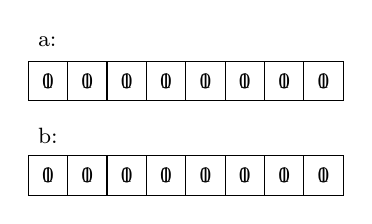
\begin{tikzpicture}
\def\x{0.5}
\def\d{0}
\foreach \i in {0,1,...,7}{
\draw (\i*\x,\d)rectangle(\i*\x+\x,\d+\x);
\ifthenelse{\i=1 \OR \i=2 \OR \i=3 \OR \i=4}
{\node at (\i*\x+0.5*\x,\d+0.5*\x) [] {\footnotesize{1}};}
{\node at (\i*\x+0.5*\x,\d+0.5*\x) [] {\footnotesize{0}};}
}
\node at (0,\d+1.5*\x) [right] {\footnotesize{a:}};

\def\d{-1.2}
\foreach \i in {0,1,...,7}{
\draw (\i*\x,\d)rectangle(\i*\x+\x,\d+\x);
\ifthenelse{\i=1 \OR \i=2 \OR \i=3 \OR \i=4 \OR \i=7}
{\node at (\i*\x+0.5*\x,\d+0.5*\x) [] {\footnotesize{1}};}
{\node at (\i*\x+0.5*\x,\d+0.5*\x) [] {\footnotesize{0}};}
}
\node at (0,\d+1.5*\x) [right] {\footnotesize{b:}};

\end{tikzpicture}
\end{figure}
\end{frame}

\begin{frame}[fragile]\ft{字符变量的存储方式}
由字符变量的存储方式可看出,可以把字符量看成是整型量。事实上,\vspace{0.05in}

\begin{itemize}
\item 
C/C++允许对整型变量赋以字符值,也允许对字符型变量赋以整型值。\\[0.1in]
\item 
在输出时,允许把字符变量按整型量输出,也允许把整型量按字符量输出。
\\[0.1in]
\item 
整型量占两个字节,字符量占一个字节。\red{当整型量按字符型量处理时,只有低八位字节参与处理。}
\end{itemize}
\end{frame}

\begin{frame}[fragile]\ft{打印字符}
  使用\lst|printf()| 打印字符,
  \begin{itemize}
  \item 若使用 \lst|%c|,将打印字符本身;
  \item 若使用 \lst|%d|,将打印对应的ASCII码。
  \end{itemize}

% \end{frame}

% \begin{frame}[fragile]\ft{打印字符}
  \pause 
\lstinputlisting[basicstyle=\ttfamily\small]
{slide03/code/charcode.c}
% \end{frame}

% \begin{frame}[fragile]\ft{打印字符}
\pause 
\begin{lstlisting}[basicstyle=\ttfamily\small]
$ gcc charcode.c
$ ./a.out
Please input a character:
A
the code for A is 65
\end{lstlisting}
\end{frame}

\begin{frame}[fragile]\ft{打印字符}
\begin{figure}
\centering
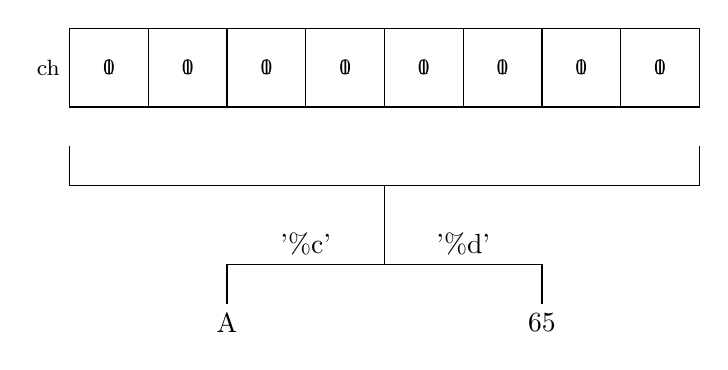
\begin{tikzpicture}
\def\x{1}
\def\d{0}
\foreach \i in {0,1,...,7}{
\draw (\i*\x,\d)rectangle(\i*\x+\x,\d+\x);
\ifthenelse{\i=1 \OR \i=6 \OR \i=7}
{\node at (\i*\x+0.5*\x,\d+0.5*\x) [] {\footnotesize{1}};}
{\node at (\i*\x+0.5*\x,\d+0.5*\x) [] {\footnotesize{0}};}
}
\node at (0,\d+.5*\x) [left] {\footnotesize{ch}};

\draw (0,-0.5*\x)--(0,-\x)--(8*\x,-\x)--(8*\x,-0.5*\x);
\draw (4*\x,-\x)--(4*\x,-2*\x);
\draw (2*\x,-2.5*\x) node[below] {A}
--(2*\x,-2*\x)
--node[above]{'\%c'}(4*\x,-2*\x)
--node[above]{'\%d'}(6*\x,-2*\x)
--(6*\x,-2.5*\x)node[below] {65};

\end{tikzpicture}
\end{figure}

\end{frame}
